 \chapter{Simulation sous Orcad Spice}
  \section{Circuit}
    Puisque notre amplificateur est composé de quatre étages indépendants, nous avons décidé d'utiliser quatre "pages"
    différentes, ainsi qu'une "page"  principale, regroupant les différents circuits précédents, afin d'y voir plus clairement.

   \subsection{Page principale}
    %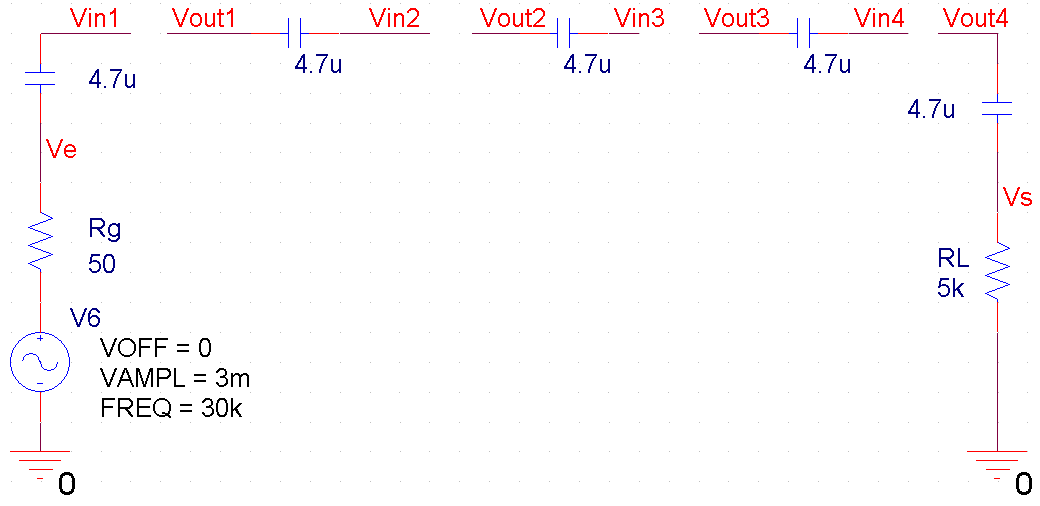
\includegraphics[width=18cm]{images/circuit_main}
    On choisit les autres condensateurs de manière à nous assurer une fréquence de coupure voisine de 100 \hertz.

   \subsection{Premier étage : Collecteur Commun}
    %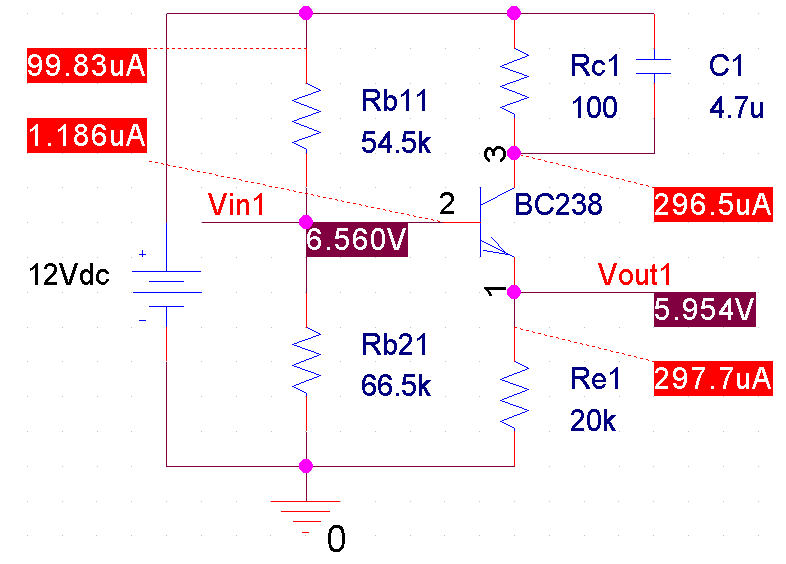
\includegraphics[width=18cm]{images/circuit_1}

   \subsection{Deuxième étage : Émetteur Commun}
    %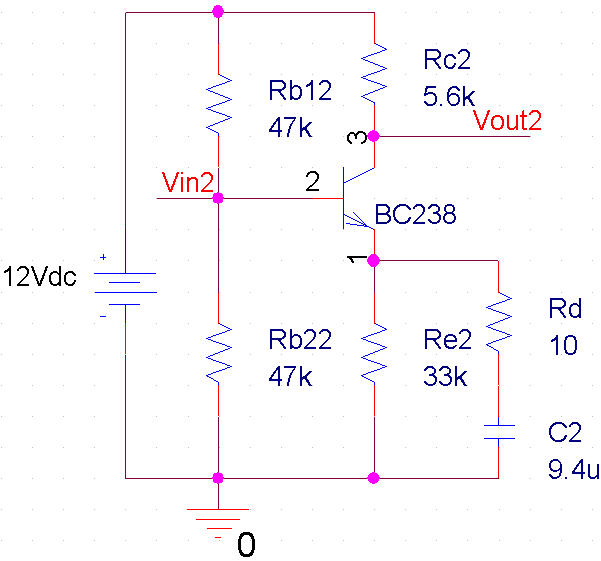
\includegraphics[width=18cm]{images/circuit_2}

    Après une première simulation sous Spice, nous nous sommes rendus compte que la fréquence de coupure basse n'était pas respectée.
    Pour cette raison, on ajoute la résistance $R_d$ en série avec le condensateur (celle-ci ne modifie pas la polarisation) afin de diminuer cette fréquence.
    Cependant, cette résistance a un fort impact négatif sur le gain, nous sommes donc amenés à augmenter la valeur du condensateur. On utilisera donc $C=9,4 \micro\farad$  ce qui correspond à deux condesateurs de 4,7 \micro\farad  en parallèle.

   \subsection{Troisième étage : Amplificateur Différentiel}
    %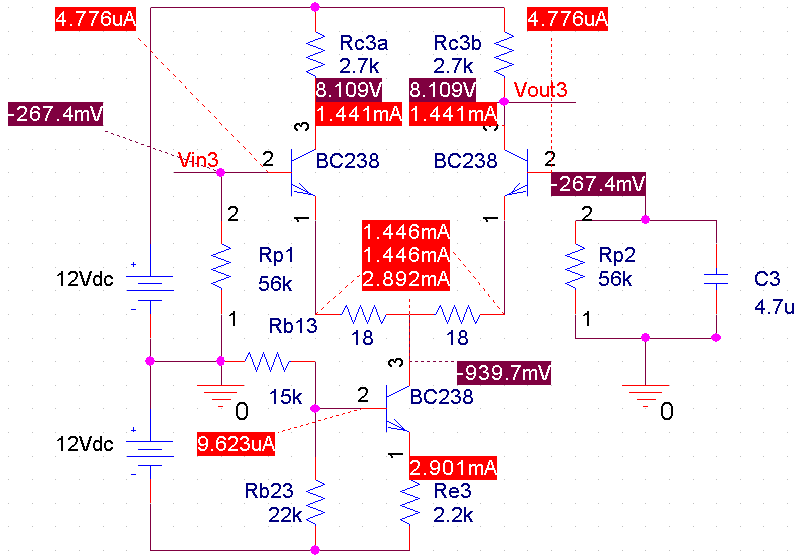
\includegraphics[width=18cm]{images/circuit_3}

    Pour cet étage, on choisira une résistance $R_p$ importante afin d'avoir un gain maximum.
    En effet celle-ci est en parallèle avec la résistance d'entrée de l'émetteur commun.

    Étant donné les mauvaises performances obtenues sur la distorsion après une première simulation, on choisit d'ajouter deux résistances de 18 \ohm  sur l'émetteur des transistors T1 et T2. Ces résistances diminuent fortement la distorsion, mais ont aussi un impact négatif très important sur le gain.

   \subsection{Quatrième étage : Collecteur Commun}
    %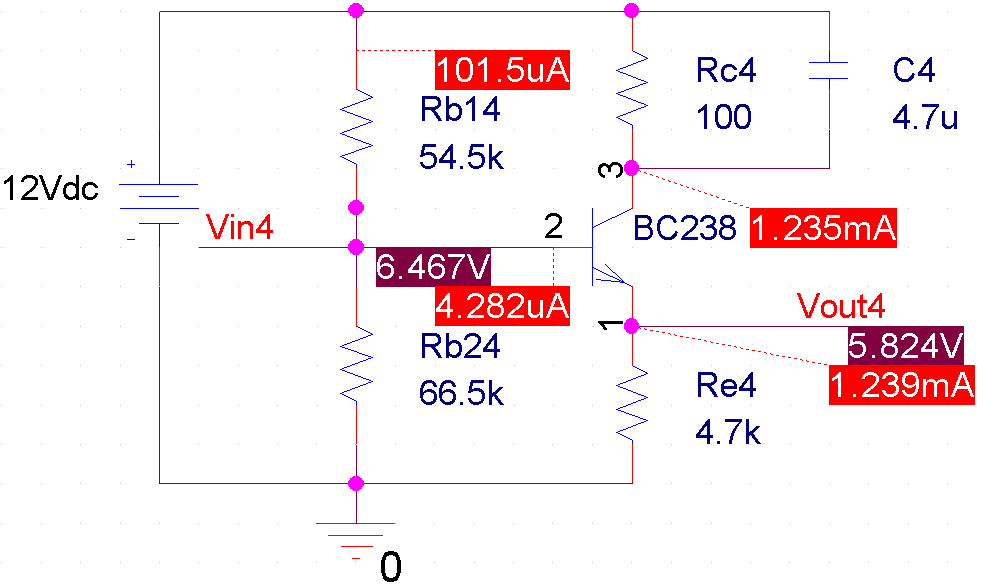
\includegraphics[width=18cm]{images/circuit_4}

  \section{Simulation}
   \subsection{Réponse temporelle à 30\kilo\hertz}
    On trace la courbe de $V_S$ en fonction du temps, et on obtient le graphe suivant, possédant une dynamique de sortie de 5,98 \volt :
    %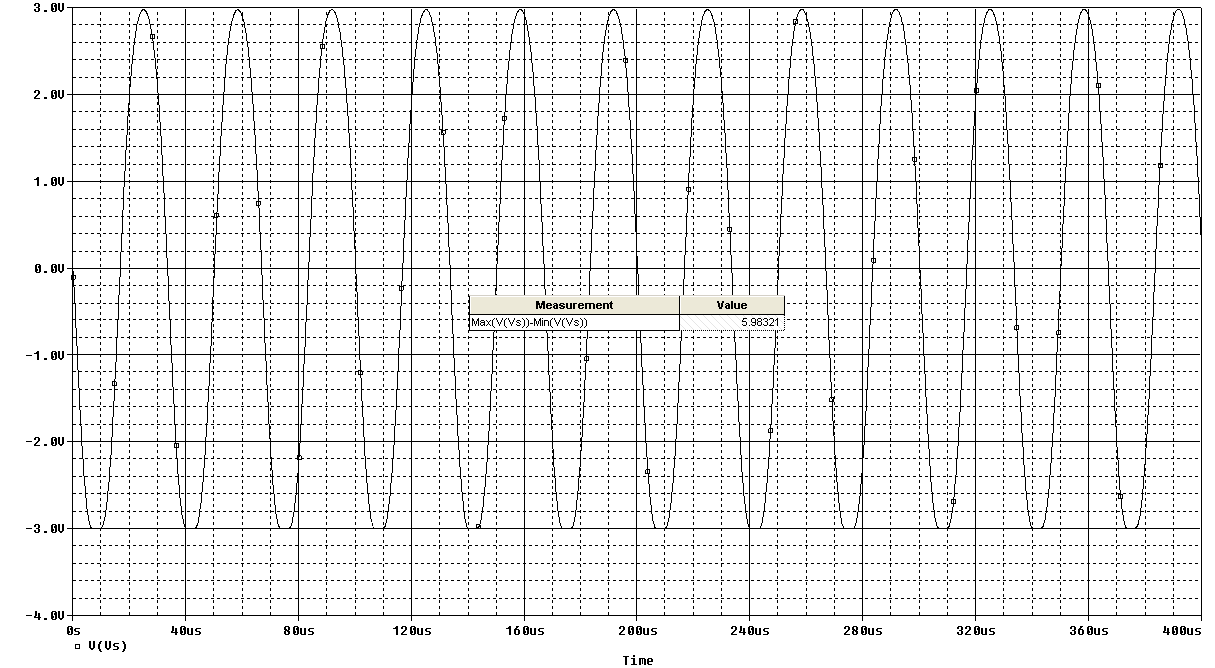
\includegraphics[width=18cm]{images/reponse_temporelle}
    
   \subsection{Diagramme de Bode}
    %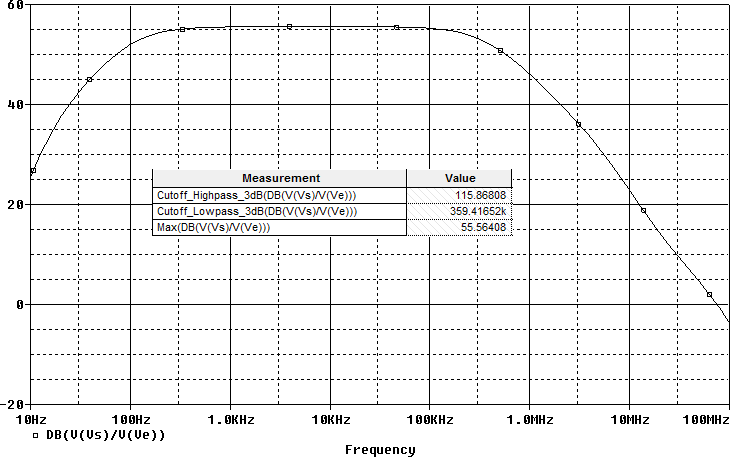
\includegraphics[width=18cm]{images/bode}

   \subsection{Transformée de Fourier}
    %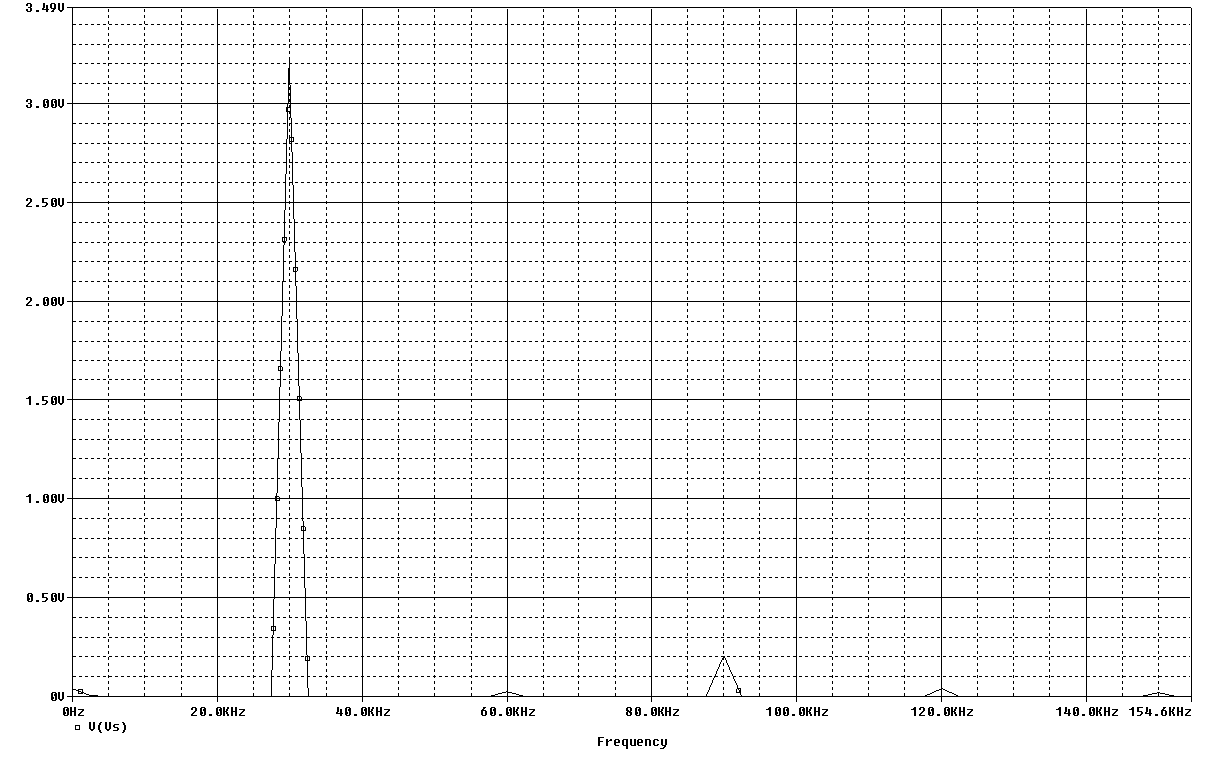
\includegraphics[width=18cm]{images/fft}

  \section{Respect du cahier des charges}
   \subsection{Fréquences de coupure}
    Ces fréquences sont données par Spice avec les fonctions \verb|Cutoff_Lowpass_3dB()| et \verb|Cutoff_Highpass_3dB()| :

    $F_{CBF} = 101$ \hertz

    $F_{CHF} = 504$ \kilo\hertz

   \subsection{Impédances d'entrée et de sortie}
    En traçant un "diagramme de Bode" sous Spice avec, pour chaque étage, $\cfrac{V_E}{I_E}$, on obtient (à 30 \kilo\hertz):
    \begin{itemize}
     \item $Z_{E_1} = \verb|29658|\ohm = Z_E$ : On respecte bien le cahier des charges.
     \item $Z_{E_2} = \verb|15034|\ohm$
     \item $Z_{E_3} = \verb|16107|\ohm$
     \item $Z_{E_4} = \verb|28788|\ohm$
    \end{itemize}

    Pour l'impédance de sortie, il faut modifier un peu le circuit sous spice : court-circuiter l'entrée et déplacer le générateur à la place de la charge. On obtient alors :
    \begin{itemize}
     \item $Z_{S_1} = \verb|191|\ohm$
     \item $Z_{S_2} = \verb|5390|\ohm$
     \item $Z_{S_3} = \verb|2690|\ohm$
     \item $Z_{S_4} = \verb|113|\ohm = Z_S \Rightarrow$ Contrairement à ce que nous avions prévu, nous n'ajouterons pas de résistance série.
    \end{itemize}

   \subsection{Gain et dynamique de sortie}
    On obtient un gain de 57.9 dB, soit une amplification de 785.
    Donc pour une dynamique de sortie de 6V, il faut une tension d'entrée de 3.8 \milli\volt.
    Or on obtient ladite dynamique de sortie avec 4.8 \milli\volt  sous Spice. Ceci est dû à une légère distorsion sur le collecteur commun du dernier étage (cf. paragraphe suivant).
   
   \subsection{Distorsion harmonique}
    Toujours d'après Spice : \verb|TOTAL HARMONIC DISTORTION =   6.668896E+00 PERCENT|

   \subsection{Courants de collecteur}
    \begin{itemize}
     \item $I_{C_1} = 0,296 \milli\ampere$
     \item $I_{C_2} = 0,162 \milli\ampere$
     \item $I_{C_3} = 1,441 \milli\ampere$
     \item $I_{C_4} = 1,235 \milli\ampere$
    \end{itemize}

   \subsection{Amplitudes crête à crête}
    \begin{itemize}
     \item $A_1 =$ \verb|9,48m| \volt
     \item $A_2 =$ \verb|242,3m| \volt
     \item $A_3 =$ \verb|5,99| \volt
     \item $A_4 =$ \verb|6,24| \volt
    \end{itemize}
